% !TeX spellcheck = en_GB
\subsection{Normative Decision Theory}
The \textbf{normative decision theory is more rational}.

The \textbf{main subject} of the normative decision theory is not
conflicting target but rather \textbf{uncertainty} (ger: Ungewissheit).\\
Often environmental conditions are also an issue when a decision has to be made.
\textbf{Environmental conditions} are factors which influence an alternative
decision over which you don't have any influence.

\mbox{}\\
In decision situations in which a certain decision is not connected to a
single possible event, a \textbf{decision involving uncertainty} is referred to.

\paragraph{Example}\mbox{}\\
If you want to a maximum of profit and you have the options to open a store
with 125,000 CHF profit and another store with 150,000 CHF, you decide
for the second one \textbf{on a rational basis}.


\subsubsection{Decision involving uncertainty}
\label{sec:decision-involving-uncertainty}
The mineral oil company is aware that a large-scale bypass is planned
but that this is highly controversial.
\begin{itemize}
	\tightlist
	\item It wouldn't affect the traffic in the town centre and the expected
	profit would remain at CHF 125,000.
	\item However, there would be a drastic change to the outskirts of town
	which would bring the expected profit down to CHF 80,000.
\end{itemize}

\subsubsection{Depiction involving uncertainty}

The \textbf{result matrix} is a tool to describe alternative actions (ai) with
different environmental conditions (zi).

\begin{figure}[H]
\centering
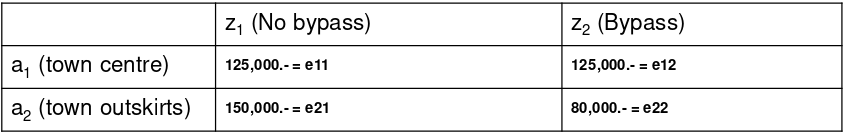
\includegraphics[width=\textwidth]{figures/resultMatrix.png}
\caption{Example of a results matrix in regard to
\secref{sec:decision-involving-uncertainty}}
\end{figure}

The decision matrix only describes the decision situation if the state
space is recorded in full. So if there are any changes of the environment in
future, you can not involve that in your decision.

\subsubsection{Classification of decision situations involving uncertainty}

\begin{description}
	\item[Decision involving risk] If occurrence likelihoods can be
	assigned to environmental conditions.
	\item[Decision involving uncertainty] If no occurrence likelihoods can be
	assigned to environmental conditions.
\end{description}

\emph{Probabilities must not only be mathematically or statistically
sound (\textbf{objective probabilities}), but rather may also only result from
the subjective view of the decision maker (\textbf{subjective probabilities}).}

\subsubsection{Decision involving probabilities}

\begin{figure}[H]
\centering
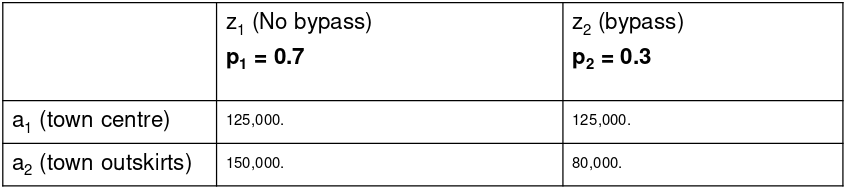
\includegraphics[width=\textwidth]{figures/resultMatrix2.png}
\caption{Results matrix with probabilities}
\end{figure}

\subsubsection{Dominance}
An alternative is described as \textbf{dominant} if it is to be
preferred over another alternative in all cases. If an alternative
dominates all others, it must be preferred on rational grounds.

\begin{description}
	\item[Absolute dominance] If the worst result value of the dominating
	alternative is better than the best result value of the dominating
	alternative.
	\item[Circumstantial dominance] One alternative in every circumstance
	(environmental circumstance) is better than (or equally good as) the
	other alternative.
\end{description}

\begin{figure}[H]
	\centering
	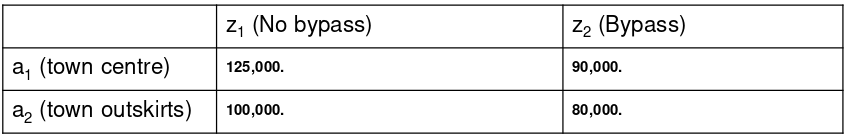
\includegraphics[width=\textwidth]{figures/absoluteDominance.png}
	\caption{Dominance example}
	\label{fig:dominance-example}
\end{figure}

In \autoref{fig:dominance-example} there is no absolute dominance, because a1 is
not better in every situation than the best of a2. There is no circumstantial
dominance, because a1 is better, regardless of the environmental conditions.

\subsubsection{Game theory}

Along with the two cases where the probabilities exist or do not exist, there
is also a third case if the environmental conditions are not determined by
coincidence but by a \textbf{rational counterpart (e.g. competing company)}.

\mbox{}\\
Generally, the occurrence of the individual environmental conditions here
can no longer be seen as independent from a person's own decision.
Situations like this are the subject of \textbf{game theory}, which represents a
special branch of decision theory.

\subsection{Decisions involving several targets}

\begin{itemize}
\tightlist
\item
  \textbf{Complementary targets}: By pursuing one target, the other
  target is also (optimally) achieved.
\item
  \textbf{Neutral targets}: Don't influence each other.
\item
  \textbf{Competing targets}: Realising one target impacts on reaching
  the other target.
\end{itemize}

\subsubsection{Efficiency of an alternative}
An alternative is efficient if there is no other alternative which is better
with regard to at least one target and not worse with regard to any target.
\begin{figure}[H]
	\centering
	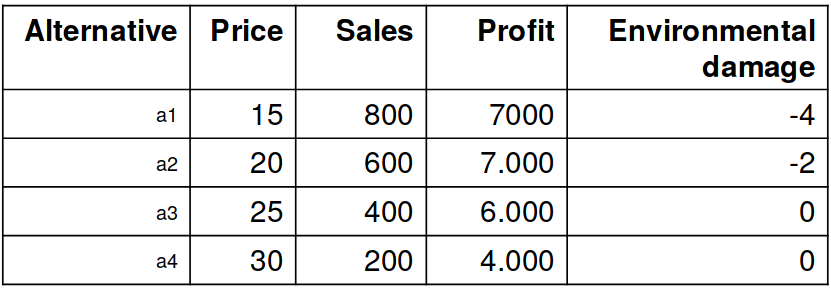
\includegraphics[width=.6\textwidth]{figures/efficiency-alternative.png}
	\caption{Example with inefficient alternative}
	\label{fig:efficiency-alternative}
\end{figure}

In \autoref{fig:efficiency-alternative} the option a4 is inefficient because
it's the most expensive choice with the lowest sales and profit.

\subsubsection{Target dominance}
If a target is considered to be the decisive one, the fulfilment of all other
targets can be put aside.

In this process, the alternative is chosen which measures best with regard
to a selected main target. In \autoref{fig:efficiency-alternative} a1 would
be chosen if the target is defined as $max(Sales)$.

\subsubsection{Lexiocographical order}

In lexiocographical order you put priorities to some criterias
(e.g.~first priority = Sales, second priority = Environmental damage).
All options will be sorted according to the priorities (primary key and
secondary key) and the one on the top wins.

\subsubsection{Utility function (Nutzwertanalyse)}

Weigthns the different parameters (e.g. the factor for profit is higher
than for revenue). Afterwards the variant with the biggest utility becomes
the chosen one.

To make this decision process work, the different parameters need to be
distributed identically (e.g. from 0-1 or 0-10).

\subsection{Decision rules}

\subsubsection{Maximin rule}

The alternative action with the maximum minimum is chosen.

\begin{description}
	\item[Intention] Decision rule with an extreme level of risk
	aversion, as only the poorest possible result is reflected in the
	evaluation.
	\item[Criticism] Not in touch with reality and only one single value
	of an alternative is taken into consideration.
\end{description}


\subsubsection{Maximax rule}

The alternative action with the maximum maximum is chosen.

\begin{description}
	\item[Intention] Extremely venturesome (optimistic) decision rule, as
	only the best possible result is reflected in the evaluation.
	\item[Criticism] Extremely out of touch with reality and equally only
	one single value of an alternative is taken into consideration.
\end{description}


\subsubsection{Hurwicz rule}

Combination of the maximin and maximax by the introduction of an
optimisation parameter lambda ($0 \le \lambda \le 1$).
\begin{equation}
\Phi(a_i) = \lambda \cdot max_j(e_{ij}) + (1-\lambda) \cdot Min_j(e_{ij})
\end{equation}
In optimistic decision making $\lambda$ should be chosen high, low otherwise.

\begin{description}
	\item[Intention] Decision rule for decision makers who are neither
	absolutely optimistic nor absolutely pessimistic.
	\item[Criticism] In	many cases out of touch with reality and only two
	values of each alternative are taken into consideration.
\end{description}


\subsubsection{Savage-Niehans rule}

Rule of the lowest regret.

\mbox{}\\
The rule attempts to minimise the maximum possible regret. Create a
regret matrix matrix in which the maxima determine the environmental
conditions and then the maximum possible difference for this value is
calculated per course of cation. The maximum possible regret is then the
row maximum.

\begin{figure}[H]
	\centering
	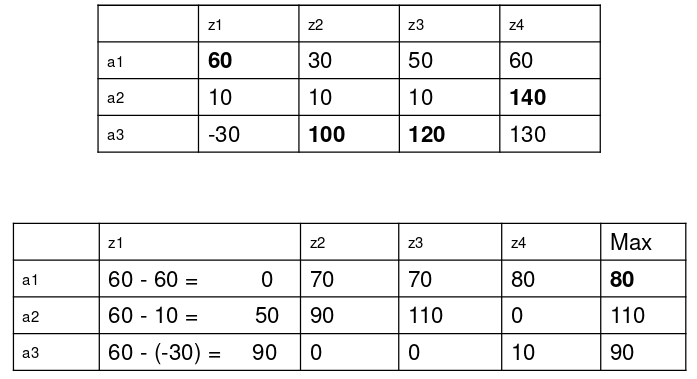
\includegraphics[width=.6\textwidth]{figures/savage-niehansRule.png}
	\caption{Example of the Savage-Niehans rule}
	\label{fig:savageniehans-rule}
\end{figure}

\textbf{You do following for each column:}\\
Take the maximum value and calculate the possible lost
value for each cell. The row (alternative) with the minimum possible
lost value (the minimum regret) wins.

\mbox{}\\
\textbf{Criticism:} With regard to the regret matrix, the decision is
based on the principles of the minimax criterion. For this reason, not
all information is used even in the case of this criterion and a
pessimistic sentiment is ultimately expressed. A particular point of
criticism relates to the circumstance that the ranking between two
alternatives can change after the addition of another alternative.


\subsubsection{Laplace criterion}

The average of all environmental conditions is formed for every
alternative. The winner is the alternative with the highest average over
all conditions.

\begin{figure}[H]
	\centering
	\includegraphics[width=0.6\textwidth]{figures/LaplaceExample.png}
	\caption{Laplace criterion example}
\end{figure}

\textbf{Criticism:} It can be said that probably most people would have
chosen the alternative a3, and thus comparing the Laplace criterion
with the other rules is more realistic.

\subsection{Logical procedure}

Subjective probabilities for environmental conditions are formed and the
decision situation is converted in this way to a decision involving
risk.

\begin{figure}[H]
\centering
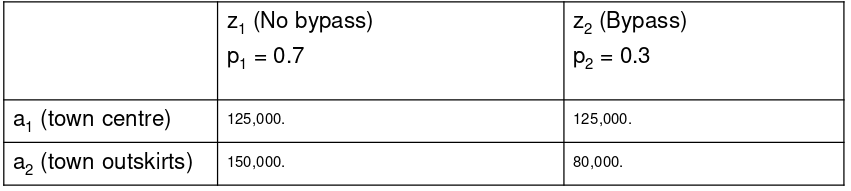
\includegraphics[width=0.6\textwidth]{figures/logicalDecisionMaking.png}
\caption{Decision involving risk}
\end{figure}

\subsubsection{$\mu$ criterion/Bayes rule}

\paragraph{Expected value} The expected value is the value which results
as a mean if the situation were to be endlessly repeated.

\begin{figure}[H]
\centering
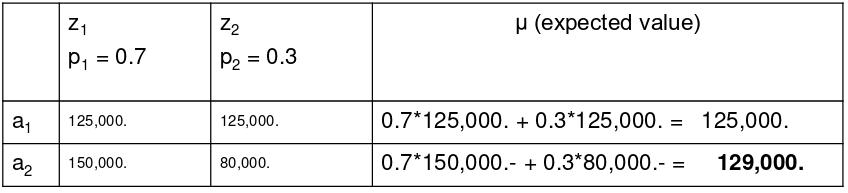
\includegraphics[width=0.7\textwidth]{figures/bayesRule.png}
\caption{Bayes rule with expected value $\mu$}
\end{figure}

\begin{description}
	\item[risk aversion] The decision maker prefers a lower expected
	value if this provides more security.
	\item[risk neutral] The decision maker prefers a lower expected
	value if this provides more security.
	\item[venturesome] The decision maker avoids a higher expected value
	in favour of a wide range of varying results.
\end{description}

\subsubsection{Decission Tree}

A decision tree always consists of one root node and any number of inner
nodes as well as at least two leaf nodes. Each node represents a logical
rule and each leaf node an answer to the decision problem.

\mbox{}\\
\emph{Decisions are drawn in square fields. Events are drawn in circles. You can also note the probability of the alternative to the related leaf or the path.}

\subsubsection{Bernoulli Principle}

The basic idea is to calculate the expected value not from the results
values but rather from the utility values and regard these as preferential
values.\\
E.g. if you get a million CHF, you can do a lot of things! But if you
earn another million (=2 MIO), you can not do the double of these
things.

\mbox{}\\
The Bernoulli survey can be used to determine the utility function,
which results in a risk-utility function (RNF) or a utility function.


\begin{figure}[H]
\centering
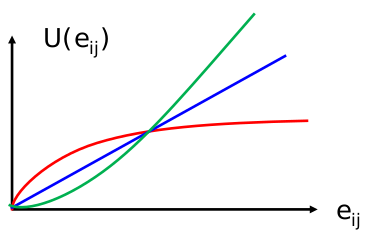
\includegraphics[width=0.3\textwidth]{figures/utilityFunction.png}
\caption{Possible utility functions. The blue is risk neutral, the green is risky, the red is risk averse.}
\end{figure}

\paragraph{Procedure}
\mbox{}\\
If the risk utility function is given, a utility or decission marix can
be formed.

\begin{figure}[H]
\centering
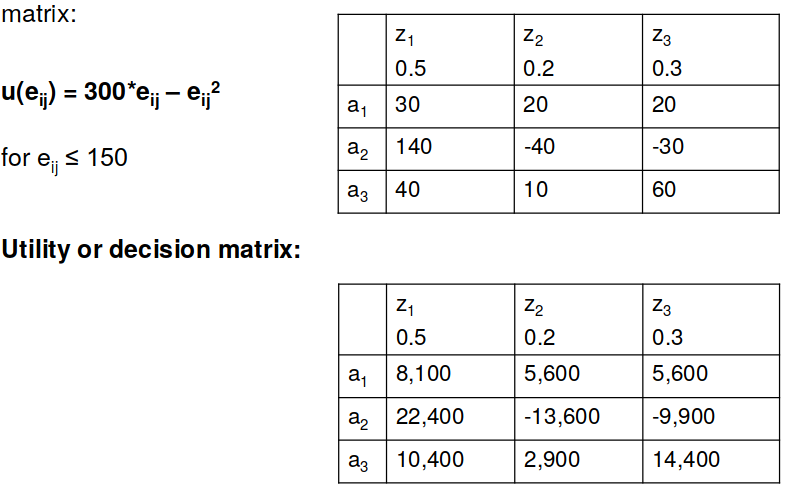
\includegraphics[width=.5\textwidth]{figures/utilitymatrix.png}
\caption{Utility Matrix}
\end{figure}

If a risk utility function is given there's only \textbf{one rational
decission}.
